\chapter{Introduction}
\label{chap:introduction}

\section{Background}
\label{section:background}

Video Generative AI\textsuperscript{[0]} is artificial intelligence models that create videos based on textual descriptions, images, or existing video inputs. \newline

This AI has been utilized in many ways, such as to use AI character models to use the product like fashion and makeup to automate advertisement, aid in generating VFX\textsuperscript{[8]}, Enhance render quality with lower-end PC\textsuperscript{[12]}, Quickly upscale videos resolution, etc.\newline

But the conception of Generative AI has been controversial in itself

It was trained with data scraped from the internet\textsuperscript{[4]}, with no regards to copyright permission or robot.txt\textsuperscript{[29]} that ask them to not use their data on their website for AI training. Of course, this sparked an outrage amongst the owner of the stolen works, who rely on commission or unique products as their main income source. Video AI is no different. Some AI engineers have been transparent on sourcing their training data only from copyright-free and ethical datasets\textsuperscript{[3]} (AnimateDiff, Adobe Firefly, Text2Video) , but the majority of the existing trained AI models\textsuperscript{[2]} does not make the separation at all (MidJourney, Sora, CogVideoX, Runway, Kling, etc.) , to the point that they openly advertised fine-tuned models that generate artwork in the style of specific artists, using their names.\newline

The widespread use of this AI has led to concerns about copyright infringement\textsuperscript{[1]}, Many artists and content creators advocate for stricter regulations to protect their works from being used without consent, to protect the future of their career. \newline

The controversy surrounding Generative AI isn’t just about copyright, it’s about how it devalues artistic labor. The issue isn’t that artists can’t produce higher-quality work, but that commissioners are willing to accept cheaper, lower-quality AI imitations that are ‘good enough’ for their purposes.\newline

However, this lack of detail and cohesion will accumulate over time, as AI operates on token-based prompts rather than true creative intent. This shift doesn’t just harm individual artists, it weakens the entire support system and foundation of the creative industry. As demand for human-made art declines, fewer aspiring artists will have opportunities to develop their skills, leading to a dwindling talent pool. Without skilled artists, industries that rely on craftsmanship such as animation, illustration, and game design will suffer, ultimately lowering the overall quality of creative work in the long run.\newline

Once that foundation is lost, rebuilding it becomes nearly impossible. Just as Disney can no longer return to the same level of hand-drawn 2D animation it once mastered after it shifted entirely to 3D animation, an overreliance on AI risks permanently degrading the artistic standards and craftsmanship that define creative industries. Without a strong base of skilled artists, industries like animation, illustration, and game design will struggle to maintain the depth and quality that set them apart in the first place.\newline

Consumers have already expressed their disappointment with the rise of AI-generated slop content, which has flooded media platforms at an overwhelming speed, pushing high-quality, human-made work out of recommendation algorithms. However, beyond AI itself, grifters\textsuperscript{[10]} have exploited this shift by infringing on copyrighted works, fine-tuning\textsuperscript{[39]} models on stolen art, and mass-producing low-effort imitations for profit.\newline

These bad actors don’t just flood platforms with AI-generated content, they actively leech off the success of original creators, diverting attention, funds, and opportunities that should have gone to real artists. As their stolen content dominates search results and recommendation feeds, genuine creators struggle to gain visibility, leading many to abandon the platform entirely.\newline

As AI-generated content continues to dominate social networks, we move closer to the so-called 'Dead Internet Theory'\textsuperscript{[11]} where authentic human interaction is drowned out by automated, mass-produced content. The internet, once a space for organic connection and creativity, is becoming increasingly hostile due to rampant exploitation, with grifters\textsuperscript{[10]} and engagement farmers prioritizing profit over meaningful discourse. If this trend continues, the internet risks becoming a hollow, artificially-generated echo chamber, devoid of genuine human expression.\newline

Lastly, One of the most alarming consequences of AI-generated video technology is impersonation\textsuperscript{[5]}, often referred to as "deepfakes\textsuperscript{[6]}." AI can create realistic videos of individuals, making them appear to say or do things they never did. This poses risks in identity theft\textsuperscript{[7]}, misinformation, fraud, and political manipulation\textsuperscript{[9]}. The ability to create hyper-realistic fake videos raises concerns about trust in digital content and calls for advanced detection methods to counteract malicious use.

Data poisoning is a method of corrupting AI models by injecting misleading or harmful data into their training sets\textsuperscript{[13]}, ensuring that generative models\textsuperscript{[14]} cannot easily exploit original artistic content. It is an aspect of data security\textsuperscript{[15]}, and restrict malicious actors from exploiting your data against your interests.

\section{Problem Statement}
\label{section:problem-statement}
The problem this project aims to solve has been well defined in the background section. \newline

As of currently, there is a solid foundation of research on the adversarial poisoning tactics\textsuperscript{[40]} against Video Generative AI, but there is currently no software that simplifies the process for common use. People may have the idea to extract the video’s graphics frame by frame, then use the existing static Image Poisoning Processor to Poison frame by frame, then reassemble them back into their video form, but there’s still technical problems, such as:

\begin{enumerate}
        \item Manually poisoning frame by frame is inconvenient for production use.
        \item Existing solution’s processing time scales horribly with video duration and fps. A 10 second video with 30 fps could take as long as 8 hours with default parameters on Glaze, and that is on the premise that the app doesn’t crash as it can only handle up to 70 images queued to poison maximum.
        \item Static Image poisoning tactics are less effective against Video generative AI.
\end{enumerate}

\section{Solution Overview}
\label{section:solution-overview}

This software seeks to simplify the process of video poisoning to be easy to use.
The software will only need the user to input their video, set some preferences, start the process and wait for the poisoned video output in their designated folder.
While being effective against generative AI and efficiently optimizing hardware resources to process larger video; ranging from 5 minutes to 2 hours, to be processed fast and reliable enough for target users such as filmmakers, content creators, and studios to incorporate this in their workflow.

\subsection{Features}
\label{subsection:features}

\begin{enumerate}[leftmargin=80pt]
    \item Video Poisoning: Poison the video by injecting perturbations\textsuperscript{[41]} that tricks the AI into learning false patterns and ruins its output consistency and quality. Before you may start, you’ll have to input your video, select the output folder, then start the poisoning process\textsuperscript{[36]}.
    \item Adjust Poisoning Parameters\textsuperscript{[15]} Settings: Set predefined Parameters such as perturbation weights\textsuperscript{[16]} or output quality\textsuperscript{[17]} to set the perturbation strength\textsuperscript{[18]} and output quality\textsuperscript{[17]}. More parameters may be added depending on the available parameters of the system's poisoning methods\textsuperscript{[19]}.
       \item Video format support: Input and Output only supports .mp4 for this project, but may add more file format supports in the future.
       \item Hardware optimization: Optimize the available hardware to minimize processing time duration. This would be done automatically but may allow users to set hardware themselves if deemed appropriate.
\end{enumerate}

\section{Target User}
\label{section:target-user}

\begin{itemize}
    \item \textbf{Digital Content Creators \& Video Artists\textsuperscript{[20]}:} They have had their creations\textsuperscript{[36]} used as training data\textsuperscript{[21]} without their permission to replicate their work, making their creative, unique, curated work being buried amongst their AI copies that hurt their profits\textsuperscript{[22]} and fame.
    \item \textbf{Industry Professionals in Media \& Entertainment\textsuperscript{[23]}:} Animation studios are at risk of having their creative works being exploited to create lower quality but faster animations. This could result in the death of the Animation industry\textsuperscript{[24]} altogether as Animator and other creatives being laid off after their works had been trained on AI and the audience ends up with an incoherent meaningless repetitive mediocre slop\textsuperscript{[25]} because the company thought that was good enough for the audience and artist become more distrustful of sharing their works online.

    \item \textbf{Anti-AI social media platforms:} Cara, BlueSky, Teezr, VGen are against any AI-generated content\textsuperscript{[26]} on their platforms. This could be part of their feature to protect their userbase’s video against being used to train on AI.
    \item \textbf{Individuals who do not want their videos to be used to train generative AI:} From the dangers of deepfakes\textsuperscript{[6]}, regular people do not want their face to be used to train generative AI in General, but data scraping was done without considering their consent. This will force data scrapers\textsuperscript{[27]} to exclude poisoned data\textsuperscript{[28]} from their training dataset\textsuperscript{[3]}.
\end{itemize}

\section{Benefit}
\label{section:benefit}
The Protractor system protects video content from non-consensual AI training\textsuperscript{[30]} by applying adversarial techniques\textsuperscript{[31]} that disrupt AI perception while remaining imperceptible\textsuperscript{[32]} to humans.

\begin{itemize}
    \item It breaks AI generated video quality and frame consistency\textsuperscript{[33]}, stopping deepfake from producing similar creations\textsuperscript{[34]}. 
    \item It enhances intellectual property\textsuperscript{[35]} protection for creators and safeguards the creative industry from AI-driven content theft\textsuperscript{[36]}.
    \item Its easy-to-use implementation allows everyone to apply AI poisoning\textsuperscript{[37]} without requiring advanced technical expertise.
\end{itemize}

\clearpage

\section{Timeline}
\label{section:timeline}
\begin{figure}[h]
    \centering
    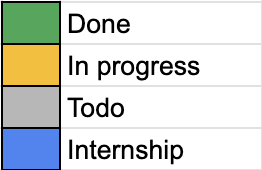
\includegraphics[width=0.5\textwidth]{chapter_1/labels.png}
    \caption{Color Meaning chart}

\end{figure}
\begin{figure}[h]
    \centering
    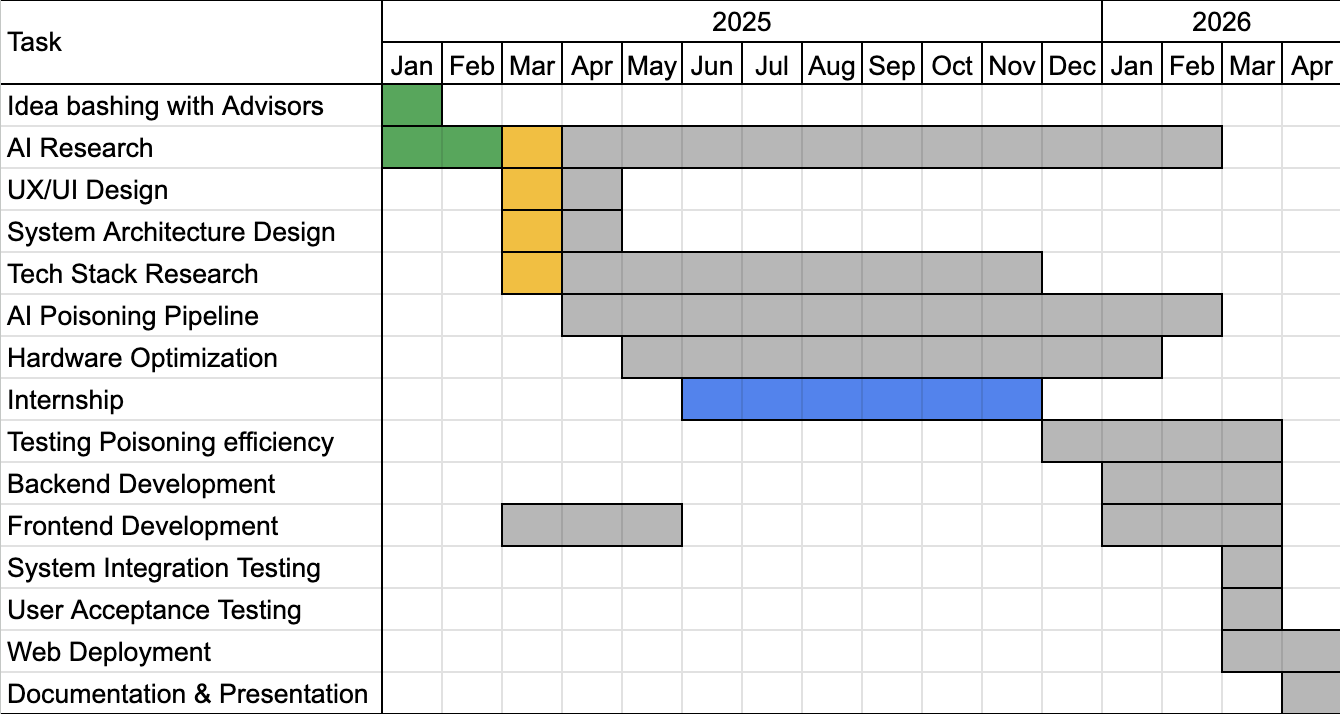
\includegraphics[width=1\textwidth]{chapter_1/timeline.png}
    \caption{Timeline of Project development}

\end{figure}

In Figure 1.2. is the current timeline of our project plan.
You may look up to Figure 1.1. for color code meanings.

\section{Terminology}
\label{section:terminology}

[0]AI : artificial intelligence \newline
[1]copyright infringement : violating copyright law over a content \newline 
[2]AI models : AI programs consisting of complex mathematical and computational techniques to process vast amounts of data and extract meaningful insights. \newline
[3]dataset : collections of data used to train AI models. \newline
[4]scraped from the internet : automatically collecting data from online sources, often using web crawlers or scrapers. \newline
[5]Impersonation : The act of fraudulently imitating a person to deceive others. \newline
[6]deepfakes : AI-generated videos that convincingly replace a person’s likeness or voice with another, often for deceptive purposes. \newline
[7]identity theft : The unauthorized use of someone’s personal information to commit fraud or other crimes. \newline
[8]VFX : Computer-generated effects used in media, often automated by AI.
[9]political manipulation : The use of deceptive tactics, such as deepfakes or AI-generated propaganda, to influence public opinion or elections. \newline
[10]Grifters : People who try to get you in get-rich-quick schemes that turned out to be a total waste of time.\newline
[11]Dead internet theory : A conspiracy introduced by IlluminatiPirate on the forum Agora Road's Macintosh Cafe esoteric board. Referring to the future where genuine human interaction is overtaken by bots and AI generated content due to the sheer amount and available.\newline
[12]lower-end PC : A computer with limited computational power, struggling with high-end tasks.
[13]poisoning tactics : The tactics of poisoning a graphics content that break AI when it trained on the poisoned piece of media content \newline
[14]static Image poisoning processor : Refer to a program that adds “AI poison” to the input non-moving image.\newline
[15]Poisoning : The process of ‘poisoning’ the input to make it break AI models when trained on, which will increase with the percentage of poisoned works in the dataset.\newline
[16]perturbation weights : perturbation is added via a formula (x + x’ = p; x is the original input, x’ is the perturbation and p is the poisoned output, x’ could be w*noise where w is weight and noise is the graphic of a randomized RGB image designed to make AI perform worse through computer vision) and added to the original image through the RGB channel of the original image.
[17]output quality : The quality of the output after the input had been poisoned\newline
[18]perturbation strength : How obvious the perturbation is in the poisoned output\newline
[19]poisoning methods : methods to ‘poison’ an image\newline
[20]Video Artists : Any artist that create video content, like animators or illustrator art timelapse where they post the process of creating their art\newline
[21]training data : data that AI trains on\newline
[22]profits : For the owner of the video, they may get their profits through commissions, platform revenue, merchandise, etc. Their profits are hurt because an AI copy could steal their originality, hard work or recommendation spots that would pay them.\newline
[23]Industry Professionals in Media and Entertainment : Refer to any creatives who work in the Media and Entertainment industry.\newline
[24]the death of the Animation industry : As the animation industry’s jobs become unstable and at risk of being replaced by AI, either the next generation of workers have to sacrifice their limited resources to compete with the availability and speed (but lack of quality) of AI, or perish. As their investors and customers use AI instead for cheaper, faster work. Jobs that could be the transition role for newbies to developing the skills of a professional are being replaced by AI, which means that there’s going to be less to no senior professional to pass the job on.\newline
[25]slop : low quality content that’s mediocre at best, but usually not good enough to provide any meaningful value to the consumer.\newline
[26]AI-generated content : Content created from AI generation via a prompt or an input image\newline
[27]data scrapers : Refer to entity that perform data scraping to collect data for any use\newline
[28]poisoned data : data that has been ‘poisoned’ that will break the AI when it was trained on.\newline
[29]robot.txt :  A file that restricts web crawlers from accessing certain parts of a site.
[30]non-consensual AI training : Refer to how AI trains on data without the data’s owner consent.\newline
[31]adversarial techniques : A data poisoning tactic where they change the data material to encourage AI to learn false patterns during backpropagation, while maintaining the perceptual similarity to the original work.\newline
[32]imperceptible : Undetectable with the human eye\newline
[33]frame consistency : How video graphics make sense between the previous, current and next frame. Low frame consistency means the video is flick-ery and objects and details appear and disappear more unpredictably.\newline
[34]similar creations : Creative products that looks similar in style or appearance\newline
[35]intellectual property : Legal rights that protect creations of the mind, such as art, music, inventions, patents, trademarks, and copyrights.\newline
[36]AI-driven content theft : Unauthorized use or replication of copyrighted materials by AI systems. It is a copyright infringement\newline
[37]AI poisoning : AI poisoning (also known as data poisoning) is a method used to corrupt or manipulate machine learning models by introducing misleading or harmful data.\newline
[38]poisoning process : The process of ‘poisoning’ the input against AI\newline
[39]fine-tuning : Adjusting a pre-trained model with specific data to specialize it.
[40]adversarial poisoning tactics : Manipulating training data to disrupt AI performance.
[41]perturbations : Small changes or modifications made to data to affect the behavior of a model, often used in adversarial attacks to mislead or deceive AI systems.
